\documentclass[times, utf8, diplomski, numeric]{fer}
\usepackage{booktabs}
\usepackage{amsmath}
\usepackage{amssymb}
\usepackage{bm}
\usepackage{algorithm}
\usepackage{algorithmic}
\usepackage{verbatim}
\usepackage{tikz,times}
\usepackage{graphicx}
\usepackage{listings}
\usepackage{color}

\definecolor{mygray}{rgb}{0.5,0.5,0.5}

\begin{document}
\thesisnumber{1136}
\title{Preporučiteljski sustavi u sveprisutnom računarstvu}
\author{Branimir Pervan}
\maketitle

% Ispis stranice s napomenom o umetanju izvornika rada. Uklonite naredbu
% \izvornik ako želite izbaciti tu stranicu.
\izvornik

% Dodavanje zahvale ili prazne stranice. Ako ne želite dodati zahvalu, naredbu
% ostavite radi prazne stranice.
\zahvala{Ovdje dolazi zahvala}

\tableofcontents

%Spomenuti IoT, recommendere i njihovu primjenu, sveprisutno računarstvo je
%prisutnije no ikad, 
%kako povezati preporučitelje i sveprisutno računarstvo, 
%što se tu ima preporučivati, koji je konkretan scenarij itd

%jednostavno, preporučiteljski sustavi filtriraju informacije iz velikih i
% nepreglednih baza podataka a gdje ćeš više informacija nego u sveprisutnom
% računarstvu koji je motiv za ovaj diplomski -> do sada se nije razvio takav
% specifičan preporučitelj
\chapter{Uvod}
U posljednjih dvadesetak godina razvoj Interneta stvari \engl{Internet
of Things} uhvatio je gotovo eksponencijalni zamah, a pojedini izvori navode da
će broj uređaja priključenih na ovu sveprisutnu mrežu do $2020$. g. doseći $26$
milijardi \cite{gartner2013Iot} odnosno $30$ milijardi \cite{ABI2013Iot}. Tomu
značajno doprinosi i konstantno opadanje cijene proizvodnog procesa tehnologije
koja naizgled obične stvari na neki način čini inteligentnima i sposobnima za
komunikaciju. 
Sveprisutno računarstvo, kao koncept u računarskoj znanosti
gdje je računarstvo prisutno svugdje \cite{theComputerWeiser}, opisuje upravo 
takve vrste stvari i uređaja, ali i takve principe gdje računalo može biti
ugrađeno u bilo kojem uređaju, na bilo kojoj lokaciji i u bilo kojem obliku.

Internet stvari samo je jedna od mogućih manifestacija sveprisutnog računarstva.

S druge strane, preporučiteljski sustavi
filtriranje sadržaja
multimedija, internetske trgovine
i ono manje primjetno, pametni prostori, arhitektura 
preporučitelji svjesni konteksta
vrijeme i prostor važni dionici konteksta

Potreba i smisao izučavanja ovog područja dolazi iz očitog primjera za
ulaganjem u bolje i efikasnije algoritme jer je u nepreglednoj masi
informacija, kakav je Internet stvari idealan izvor, procesna moć današnjih
računala davno izgubila bitku.

Dodano u uvod

Motiv ovog diplomskog rada jest manjak dostupnih algoritama za ovakvu
specifičnu vrstu preporučitelja. U ovom radu dat će se teorijska
podloga bazičnih algoritama za filtriranje sadržaja te analizirati prednosti i
nedostatke takvih pristupa. Prikazat će se principi primjene preporučiteljskih
sustava u sveprisutnim aplikacijama te će se prikazati i analizirati posebni
zahtjevi na preporučiteljske sustave od strane takvih aplikacija na konkretnom
scenariju. Na kraju će biti dan prikaz razvijenog preporučiteljskog sustava za
takvu primjenu.

\chapter{Sveprisutno računarstvo}
\section{Uvod u sveprisutno računarstvo}
A šta koji drek ovdje da pričam. Što je sveprisutno računarstvo, tko ga je
definirao, što u njemu dolazi do izražaja, koje su koristi?

Termin \glqq Sveprisutno računarstvo\grqq prvi je upotrijebio Mark Weiser u
svom vizionarskom članku u kojem je rekao kako su najkorisnije
one one tehnologije koje nestaju, u smislu da korisnici izgube pojam o
korištenju te tehnologije \cite{computer21}. 

Cilj filozofije sveprisutnog računarstva nije staviti čovjeka u svijet računala
nego integracija računala u svijet čovjeka. Praktična posljedica toga jest
pojava velike količine mahom nestrukturiranih podataka koje mogu predstavljati
izvrstan materijal za daljnju obradu i izučavanje algoritama kojima se ti podaci
mogu upotrijebiti za analizu ponašanja čovjeka ili za pomoć u svakodnevnim
poslovima \cite{VukoticTankovic}.



\section{Razvoj}
U općem slučaju mogu se razlikovati tri velika vala u računalnoj eri. To su:
\begin{enumerate}
  \item Radne stanice \engl{Mainframe} - jedno računalo, više osoba
  \item Osobna računala \engl{PC, Personal Computer} - jedno računalo, jedna
  osoba
  \item Sveprisutno računarstvo \engl{Ubiquitous Computing} - više računala,
  jedna osoba
\end{enumerate}

\begin{figure}[!htb]
	\centering
	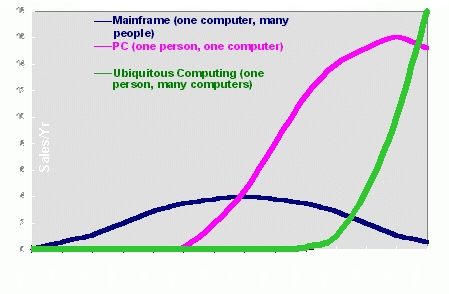
\includegraphics[width=10cm]{images/majortrends.png}
	\caption{Tri vala u računarstvu (preuzeto u edukacijske svrhe, ne valja slika)}
	\label{fig:majortrends}
\end{figure}

\section{Zahtjevi}
Analiziranjem zahtjeva na sveprisutno i prožimajuće računarstvo, može se
zaključiti nešto:
\begin{itemize}
  \item Mali uređaji
  \item Umrežavanje
  \item Sakupljanje podataka i razmjena u okruženju bez prisustva korisnika
  \item Otvoreno računarstvo radi podložnosti promjene softwarea i uređaja
  (Java ili CLR ili nekaj takvo -> bytecode)
\end{itemize}

Još jedna lista zahtjeva na sveprisutno
\begin{itemize}
  \item Uređaj za prikaz, terminal, korisnički interface
  \item Ekonomična cijena
  \item Širok mrežni opseg
  \item Sistem nevidljivih datoteka (bez znanja o direktorijima, nazivu
  datoteka, lokaciji td.)
  \item Automatska instalacija - migracija s jednog računala na drugi
  \item Personaliziranost informacija
  \item Privatnost (ima puno personaliziranih informacija, što ako se netko
  dokopa?)
\end{itemize}

koje su glavne potrebe za rad sa sveprisutnim sustavima (mala energija,
procesna moć, interakcija s okolinom)

\section{Primjena}

Udri brigu na veselje u ovom poglavlju natuć za sva vremena xD

Pametni gradovi, pametni prostori, internet stvari.

Aspekt integracije: postojeće stvari -> nova tehnologija (orjentacija u muzeju
s mobitelom)

Primjene u urbanom računarstvo:
\begin{itemize}
  \item Javne i komercijalne infrastrukture
  \item Mobilne i druge bežične mreže
  \item Kolektivni transport
  \item Plaćanje
  \item Sigurnost i nadgledanje
  \item Rasprostranjeno reklamiranje
  \item Pametna arhitektura
  \item Spektakularni urbani događaji
  \item Mobilni tehnološki uređaji
  \item Osobna komunikacija
  \item Servisi socijalnih mreža
  \item Urbana umjetnost?
\end{itemize}

Urbani krajolik -> skriveni slojevi mogu postati vidljivi, svojevrsni izum
mikroskopa.

Urbano računarstvo -> ljudi koji žive u urbanoj stredini mogu imati mnogo
različitih interesa ali imaju jednu stvar koja im je zajednička: mjesto gdje
žive (ovo bi se moglo primjeniti na činjenicu da svi imaju isti cilj u šopingu)

\chapter{Preporučiteljski sustavi}
\section{Uvod u preporučiteljske sustave}
Preporučiteljski sustavi su, ukratko rečeno, podrazred sustava za filtriranje
podataka kojima je svrha predviđanje ocjene (ili preferencije) kojom bi neki
korisnik ocijenio neki predmet u sustavu \cite{RSHandbook} Predmeti nad kojima
takvi sustavi rade, kao i korisnici tog sustava opisani su određenim
karakteristikama, odnosno važnostima tih karakteristika za korisnike. Općenito,
može se reći da je jednostavan model preporučiteljskog sustava dan formulom:
\begin{equation}
\label{eq:elementarniModel}
	R \leftarrow U \times I
\end{equation}
gdje je $R$ rezultat, tj. predikcija \engl{prediction, recommendation},
ocjene korisnika $U$ \engl{ user} koji je zatražio preporuku, tj. filtriranje
sadržaja , a $I$ predmet nad kojim se vrši predikcija ocjene \engl{item}.
Drugim riječima, predikcija je posljedica karakteristike, tj. preferencije
korisnika, te karakteristike predmeta. Traženje potencijalnih preporuka za
korisnika $U$ tada se u najjednostavnijem slučaju svodi na kombiniranje profila
njegovih preferencija s profilima predmeta u skupu svih predmeta dostupnih
algoritmu za filtriranje.
Dakle, preporuka $R$ zapravo je predviđanje ocjene korisnika $U$ za
traženi predmet $I$. Krajnji rezultat na kraju jest najčešće lista od $n$
najboljih preporuka, tj. pretpostavki da bi korisnik te predmete ocjenio
najbolje \engl{top -- $N$ list}. 

Gornji model ima dva osnovna i lako uočljiva ograničenja:
\begin{enumerate}
  \item Traženje preporuka za korisnika svodi se na iscrpno pretraživanje
  prostora predmeta dostupnih algoritmu za filtriranje
  \item Rezultat je preporuka kojoj fali bilo kakav kontekst.
\end{enumerate}

U svrhu riješavanja gore navedenih problema, razmotrit će se razni modeli
preporuke od kojih su neki već dobro poznati i korišteni algoritmi. Neka je $C$
kontekst u kojem korisnik $U$ traži preporuku. Formula \ref{eq:elementarniModel}
tada prelazi u:
\begin{equation}
\label{eq:elementarniModelSKontekstom}
	R \leftarrow U \times I \times C
\end{equation}
dok predikcija $R$ postaje posljedica karakteristike, tj. preferencije
korisnika, karakteristike predmeta i konteksta u kojem se vrši predikcija.
Kontekst $C$ se ne shvaća atomarno i u sebi može sadržavati više različitih
komponenata koje mogu utjecati na preporuku, npr:
\begin{itemize}
  \item Vrijeme predikcije
  \item Mjesto na kojem se traži predikcija
  \item Prisutnost drugih korisnika u trenutku predikcije
  \item Skupine predmeta, odnosno resursa, koje se nalaze u blizini
\end{itemize}

Predmet se shvaća generički i on može varirati ovisno o kontekstu primjene,
primjerice, artikli u internet trgovini, knjige u digitalnim knjižnicama, pjesme
i filmovi namultimedijalnim servisima, rezultati pretraživanja na tražilicama,
osobe na društvenim mrežama, smjerovi kretanja u prostoru i u ovisnosti s
vremenom itd. Svaki predmet u korišten od strane algoritma za filtriranje obično
je opisan nekim karakteristikama koji variraju u ovisnosti o kontekstu predmeta.
Tako primjerice neka pjesma može biti opisana žanrom, trajanjem i izvođačem, a
knjiga isto tako žanrom, autorom i brojem stranica. Unositi težine za pojedine
ocjene karakteristika predmeta nije uobičajeno jer na taj način dolazi do
subjektiviziranja rezultata filtriranja na manji skup osoba, ali s druge strane
gledano, nije ni nemoguće.

S druge strane, korisnici sustava imaju različite scenarije korištenja
preporučitelja od kojih su osnovni filtriranje neželjenog sadržaja iz velikih
baza podatak i savjetovanje pri nedostatku vlastite kompetencije za izbor
sadržaja \cite{AskIda}. Korisnici imaju svoje preferencije koje su u ovom
slučaju uglavnom opisane težinama jer prema različitim potrebama određene
karakteristike predmeta nad kojima se vrši filtriranje mogu biti zanimljivije,
odnosno manje zanimljive.
%TODO: SVD tu negdje?

Interakcijom korisnika sa sustavom omogućuje se praćenje njegovih odabira,
treniranje preporučitelja te kroz analizu profila korisnika i njegovih osobnih
preferencija stvaranje modela za preporuku predmeta na nekoliko načina. Podaci
koje korisnik ostavlja u sustavu u osnovi se mogu podijeliti u dva skupa:
\begin{enumerate}
  \item Implicitni
  \item Eksplicitni
\end{enumerate}
Implicitni podaci su oni podaci koje je sustav prikupio od korisnika bez da ga
je to eksplicitno zatražio. Takvi podaci mogu biti primjerice, demografski
podaci, točnije, šire područje iz kojeg korisnik koristi sustav a jednostavno se
doznaje iz baze podataka dodijeljenih područja \engl{scope} IP adresa.
Također, pod implicitne podatke spadaju i akcije korisnika u sustavu koje se
mogu doznati iz sjedničkih zapisa, kao i tzv. klikovi na određene poveznice
unutar sustava.

S druge strane, eksplicitni podaci su oni koje korisnik ostavlja s namjerom,
primjerice koristeći ankete o svojim preferencijama, ostavljajući povratnu
informaciju na ponuđene predmete \engl{feedback} ili odgovarajući na bilo
koji način na upite o pojedinim predmetima.

U općem slučaju, preporučiteljske sustave razlikujemo prema načinu filtriranja i
analiziranja informacija, a razlikujemo četiri osnovna načina:
\begin{enumerate}
  \item Filtriranje neovisno o korisniku \engl{Non -- personalized
  filtering}
  \item Filtriranje zasnovano na sadržaju \engl{Content -- based
  filtering}
  \item Filtriranje zasnovano na suradnji \engl{Collaborative
  filtering}
  \item Hibridne tehnike filtriranja odnosno preporučivanja
\end{enumerate}
Iako se tehnički iz filtiranja neovisnog o korisniku može izgraditi
preporučiteljski sustav, on to nije u punom smislu riječi jer praktički
izostavlja ulogu korisnika u sustavu. Drugim riječima, svaki korisnik će dobiti
istu preporuku. Zbog toga ga se može nazvati svojevrsnim
\emph{pseudopreporučiteljem}.

\section{Razvoj preporučiteljskih sustava}
Povijesno gledano, razvoj preporučiteljskih sustava započeo je devedesetih
godina prošlog stoljeća, a nemalo je populariziran $2006$. g. svojevrsnim
natjecanjem \glqq The Netflix Prize \grqq kada je poznati pružatelj multimedije
na zahtjev ponudio nagradu od \$$1,000,000$ američkih dolara za tim koji razvije
preporučitelj bolji od taga postojećeg sustava \glqq Cinematch \grqq za određeni
postotak \cite{Bennett2007}.
Ovo je ostavilo velik utjecaj na razvoj preporučitelja prvenstveno zbog
činjenice da je u uvjetima natjecanja navedeno da rezultati i principi rada
razvijenih preporučitelja moraju biti javno objavljeni i dostupni
%referenca

\section{Filtriranje neovisno o korisniku}
%TODO negdje ubaciti kako zapravo dobiti preporuku (top N)
Osnovni model filtriranja jest filtriranje neovisno o korisniku. Model preporuke
koji proizlazi iz ovakvog načina filtriranja, strogo gledano, ne može biti
preporučitelj jer preporuka ne ovisi strogo o korisniku. Drugim riječima, svaki
korisnik koji zatraži preporuku od ove vrste filtriranja dobit će istu
preporuku. Ova tvrdnja može se jednostavnije prikazati relacijom:
\begin{equation}
\label{eq:filtriranjeNeovisnoOKorisniku}
	R \leftarrow I
\end{equation}
gdje je $R$ predikcija, tj. preporuka, a $I$ predmet. Iz relacije
\ref{eq:filtriranjeNeovisnoOKorisniku} očigledno je da je predikcija funkcija
isključivo predmeta, pa kao takva ne može biti smatrana punokrvnim
preporučiteljem. S druge strane, isplati se proučiti ovu vrstu filtriranja jer
neki njezini koncepti vrijede u općem slučaju, npr. sustav ocjenjivanja i sustav
prikazivanja rezultata.

Razmjerno jednostavna predožba ovog modela jest rejting \engl{Rating}. Neka je
dan neki servis za ocjenjivanje i korisničke recenzije ugostiteljskih objekata.
Neka svaki korisnik koji je koristnio uslugu nekog od objekata ima pristup
sustavu u kojem može u više kategorija ostaviti ocjenu iz nekog intervala s
pisanom recenzijom. Također, neka svaki korisnik ima mogućnost ocijeniti uslugu
brojčanom ocjenom iz intervala od jedan do pet. Model preporučitelja u tom
slučaju je opisan s:
\begin{equation}
\label{eq:skupOcjena}
	S = \{1, 2, 3, 4, 5\}
\end{equation}
\begin{equation}
\label{eq:prosjek}
	R = \lfloor \frac{\sum_{i=1}^{N} s_i}{N} \ast 10 \rfloor
\end{equation}
gdje je $S$ skup mogućih ocjena, $R$ konačan rejting predmeta, $N$ ukupan broj
korisnika koji su ocjenili taj predmet, a $s_i$ ocjena $i$-tog korisnika. Iako
izgrađeni model preporuke strogo gledano nije preporučitelj, on to ipak čini
posredno nudeći korisniku ono što su drugi korisnici obilježili kao poželjnije.
Ovakav model obično koriste usluge s povratnom informacijom korisnika
\engl{Feedback}, npr. \emph{eBay}, \emph{Tripadvisor} i \emph{Zagat}.

\begin{figure}[!htb]
	\centering
	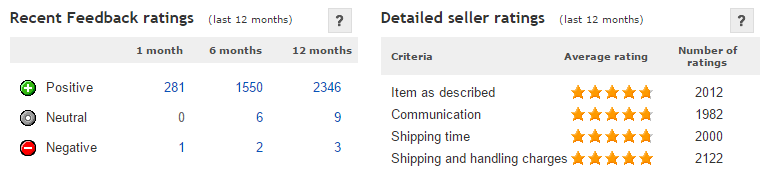
\includegraphics[width=14.21cm]{images/neosobni/ebay1.png}
	\caption{Primjer rejtinga na internetskoj aukcijskoj kući \emph{eBay}}
	\label{fig:Ebay1}
\end{figure}

Elementi ovog preporučitelja prikazani relacijama \ref{eq:skupOcjena} i
\ref{eq:prosjek} mogu se varirati kako bi se prilagodio izgrađeni model drugim
sustavima, primjerice:
\begin{itemize}
  \item Skup ocjena $S$. Ovisno o potrebi, moguće je skup proširiti do potrebnog
  broja ocjena, imajući na umu da veća granulacija nije nužno bolja, kao i da
  može biti beskorisna u vidu onemogućenja korisnika da predmet ocjeni spontano,
  a da neće biti vidljiva u krajnjem rezultatu. Također, granulaciju je moguće
  povećati dozvoljavanjem ocjena van skupa cijelih brojeva.
  \item Prikaz rezultata $R$. U formuli \ref{eq:prosjek} prije zaokruživanja
  prosjek je pomnožen faktorom $10$ radi eliminacije decimala. Moguće je
  odabrati neki drugi prikaz rezultata, primjerice u postotcima (slika
  	\ref{fig:Ebay2}).
\end{itemize}
Preporuka korisniku na kraju se jednostavno svodi na prikaz prvih $N$ najboljih
prosječnih ocjena.

\begin{figure}[!htb]
	\centering
	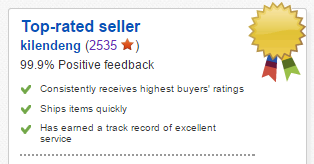
\includegraphics[width=5cm]{images/neosobni/ebay2.png}
	\caption{Implicitna preporuka trgovca izražena postotcima}
	\label{fig:Ebay2}
\end{figure}

Sam način ocjenjivanja ne mora nužno biti eksplicitna dodjela ocjene. Moguće je
primjerice koristiti sustav glasovanja \engl{Vote up/down} \engl{Vote
up/down}. Pomoću takvog sustava, korisnici masovno određuju koji je sadržaj
kvalitetniji, odnosno, koji je manje kvalitetan te na taj način vrše implicitnu
preporuku. Primjer je internetska stranica za programerska pitanja i odgovore
\emph{StackOverflow} (slika \ref{fig:stackoverflow1}). Na ovoj stranici, nakon
postavljenog pitanja, korisnici daju odgovore, a sustav na više pozicije
postavlja one odgovore kojima su korisnici dali više glasova, a na niže pozicije
lošije i negativno rangirane odgovore. Također, korisnici mogu glasovati na
kvalitetu postavljenog pitanja pa time nekvalitetna i loše postavljena pitanja
eliminirati (tj. ne preporučiti) za odgovaranje. 

\begin{figure}[!htb]
	\centering
	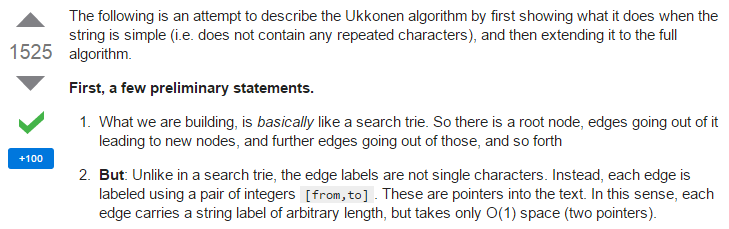
\includegraphics[width=14.21cm]{images/neosobni/stackoverflow1.png}
	\caption{Primjer rejtinga na internetskom portalu \emph{StackOverflow}}
	\label{fig:stackoverflow1}
\end{figure}

Drugi najpoznatiji primjer koji koristi takav sustav dodjele ocjena jest
internetski portal \emph{Reddit} (slika \ref{fig:reddit1}).
\begin{figure}[!htb]
	\centering
	
\includegraphics[width=14.21cm]{images/neosobni/reddit1.png}
	\caption{Primjer rejtinga na internetskom portalu \emph{Reddit}}
	\label{fig:reddit1}
\end{figure}

%TODO: Ovo kao da je nabacano, i ovo iznad i ovo ispod ove linije?
U općem slučaju modeli preporučitelja zasnovani na ovakvoj vrsti filtriranja
imaju dvije mane:
\begin{itemize}
  \item Zavaravanje korisnika od strane rejtinga koji je, neovisno o načinu
  prikaza, i dalje samo prosjek pojedinačnih ocjena.
  \item Nedostatak konteksta za preporuke.
\end{itemize}

Nepersonalizirana preporuka može se izvesti i asocijativno, traženjem implicitne
korelacije između dvaju ili više predmeta. Naivno gledano, može se zaključiti
ako je relativna većina korisnika uz kupnju nekog proizvoda $i_1$ kupila i
proizvod $i_2$, da bi i budućim korisnicima trebalo uz proizvod $i_1$
preporučiti proizvod $i_2$, i obrnuto. Ova tvrdnja može se opisati formulom
\ref{eq:NaivnaNep}:

\begin{equation}
\label{eq:NaivnaNep}
	R = \frac{\mid X \cap Y \mid}{\mid X \mid}
\end{equation}
gdje je $X$ skup svih korisnika koji su kupili predmet $i_1$, $Y$ skup svih
korisnika koji su kupili predmet $i_2$ a $R$ ocjena ovisnosti između predmeta
$i_1$ i $i_2$. Zbog činjenice da je kardinalni broj presjeka dvaju skupova
uvijek manji ili jednak kardinalnom broju bilo kojeg od ta dva skupa, ocjena $R$
nalazi se u intervalu $0 \leq R \leq 1$.

Problem ove metode preporučivanja jest navedeni nedostatak konteksta za
preporuke. Taj nedostatak može se manifestirati u činjenici da su neki predmeti
neovisno popularni. Primjerice, ako je neki predmet popularan, naivni
preporučitelj može koristeći \ref {eq:NaivnaNep} (opravdano) stvoriti vezu
između tog predmeta i bilo kojeg drugog predmeta. Primjer dan u
\cite{courseraRC} pokazuje kako su u nekom sustavu posebno popularan predmet
banane i kako naivni preporučitelj stvara veze između banana i nekih drugih
generičkih predmeta, pa onda pri kupnji banana preporučuje te generičke predmete
i obratno. Ovaj efekt može se eliminirati normalizacijom relacije
\ref{eq:NaivnaNep}:

\begin{equation}
\label{eq:nepersonalizirani}
	R = \frac
		{\frac
			{\mid X \cap Y \mid}
			{\mid X \mid}}
		{\frac
			{\mid \overline{X} \cap Y\mid}
			{\mid \overline{X} \mid}}
\end{equation}
gdje su $X$ i $Y$ skupovi svih korisnika koji su kupili predmete $i_1$ i $i_2$
respektivno.

\section{Filtriranje ovisno o korisniku}
Grubi model filtriranja ovisnog o korisniku, prema relaciji
\ref{eq:elementarniModel} računa predikciju kao produkt karakteristike predmeta
i preferencije korisnika, no zanemaruje kontekst, osim ako on nije implicitno
uključen u komponentu korisnika ili predmeta. U općem slučaju razlikuju se dvije
vrste filtriranja ovisnog o korisniku: filtriranje zasnovano na sadržaju te
suradničko filtriranje.

\subsection{Filtriranje zasnovano na sadržaju}
U gotovo svim primjenama preporučitelja, tj. u sustavima u kojima se oni
koriste, predmeti ili korisnici nisu osnovne (atomarne) jedinice, nego ih se
može opisati nekim kategorijama, primjerice, demografskim podacima za korisnika,
autorom i izdavačem ako je predmet neka knjiga i sl. Preporučivanje zasnovano
na sadržaju u osnovi dovodi u vezu prikupljene preferencije korisnika, bilo
eksplicitno, bilo promatrajući povijest ponašanja, i karakteristike kojima je
opisan neki predmet \cite{RSHandbook}. Na slici \ref{fig:contentnonpers} vidljiv
je primjer preporučiteljskog rezultata bez ikakvih informacija o korisniku.

\begin{figure}[!htb]
	\centering
	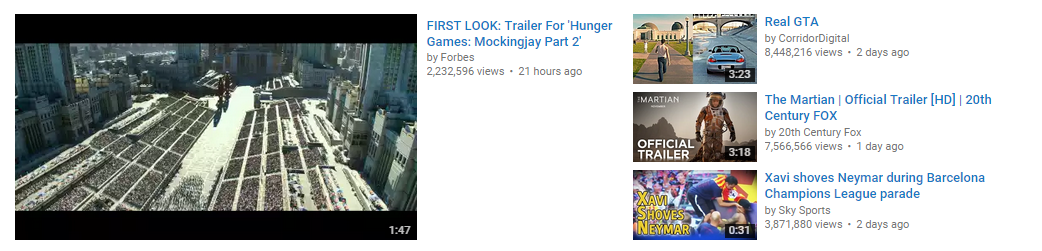
\includegraphics[width=14.21cm]{images/content/nepersonalizirani.png}
	\caption{Preporuka zasnovana na sadržaju i implicitno prikupljenim podacima}
	\label{fig:contentnonpers}
\end{figure}

Podaci na temelju kojih je generirana preporuka prikupljeni su implicitno, u
vidu grube lokacije korisnika (na slici je lokacija Ujedinjeno Kraljevstvo). S
druge strane, slika \ref{fig:contentpers} prikazuje uključene podatke o
korisniku, pa je lako vidljiva značajna razlika u generiranoj preporuci između
dvije verzije preporučitelja u kojoj isti algoritam ima pristup različitim
širinama skupova informacija. 

\begin{figure}[!htb]
	\centering
	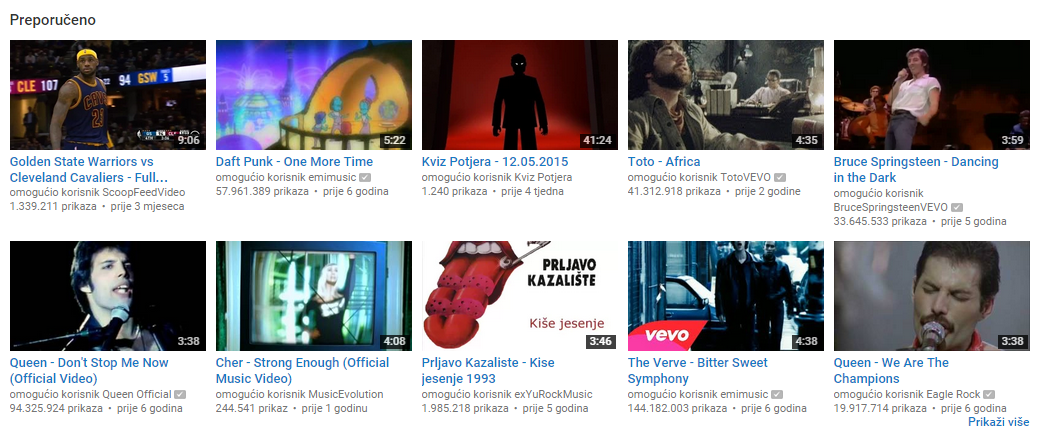
\includegraphics[width=14.21cm]{images/content/personalizirani.png}
	\caption{Preporuka zasnovana na sadržaju i eksplicitno personalizirana}
	\label{fig:contentpers}
\end{figure}

Neka je u sustavu koji koristi preporučitelj zasnovan na sadržaju svaki predmet
opisan tekstualnim medapodacima i vektorom:
\begin{equation}
\label{eq:vektorKarakteristika}
	\boldsymbol{X_i} = 
		\big[ 
			\boldsymbol{w_{1,i}}, 
			\boldsymbol{w_{2,i}}, 
			\boldsymbol{w_{3,i}}, 
			\ldots, 
			\boldsymbol{w_{N,i}} 
		\big]^T
\end{equation}
gdje je $\boldsymbol{w_{j,i}}$ kvantitativni, tj. brojčani opis neke $j$-te
karakteristike za $i$-ti predmet. Težina je neka proizvoljno odabrana metrika
koja može varirati od jednostavnog broja pojavljivanja, uključujući $0/1$
pristup (karakteristika je primjenjiva, odnosno karakteristika nije
primjenjiva) do precijznijih metrika. Sličnost između dvaju predmeta, $i_1$ i
$i_2$ moguće je tada izraziti kosinusom kuta između vektora njihovih
karakteristika:
\begin{equation}
\label{eq:kosinus}
	\boldsymbol{cos}(\boldsymbol{I}_1, \boldsymbol{I}_2) = 
		\frac
			{\boldsymbol{I}_1 \ast \boldsymbol{I}_2}
			{\|\boldsymbol{I}_1\| \times \|\boldsymbol{I}_2\|}
\end{equation}
Teoretski, svaka karakteristika može imati svoju težinu, u smislu da može biti
važnija, odnosno manje važna za opis nekog predmeta. Taj pristup svodi se na
algoritam \emph{Redukcije dimenzija} i dekompoziciju matrice na singularne
faktore, a bit će opisan naknadno.

Neka također za svakog korisnika postoji korisnički profil sa dostupnim
preferencijama korisnika dostupnim u vektorskom zapisu gdje $i$-ta komponenta
vektora predstavlja težinu te karakteristike za korisnika. Tada je na sličan
način moguće izraziti kompatibilnost promatranog korisnika i predmeta:
\begin{equation}
\label{eq:cosUserItem}
	\boldsymbol{cos}(\boldsymbol{U}, \boldsymbol{I}) = 
		\frac
			{\boldsymbol{U} \ast \boldsymbol{I}}
			{\|\boldsymbol{U}\| \times \|\boldsymbol{I}\|}
\end{equation}

%TODO: ubaciti TFIDF

Vektore je poželjno normalizirati, TFIDF

S obzirom na relacije \ref{eq:kosinus} i \ref{eq:cosUserItem} slijedi algoritam
za preporučivanje zasnovano na sadržaju:

\begin{algorithm}[!htbp]
	\caption{Filtriranje zasnovano na sadržaju}
	\label{algo:content}
	\begin{algorithmic}[1]
		\STATE{\textbf{Ulaz:} $k$ - vektor ocjena korisnika. $I$ - matrica u kojoj su
		retci predmeti, a stupci karakteristike}
		\STATE{\textbf{Izlaz:} Lista $L$ najboljih $N$ predmeta za korisnika $k$}
		\STATE{$L := initList(N)$}
		\STATE{$idfPolje := initPolje(width(I))$}
		\STATE{$userPolje := initPolje(width(I))$}
		
		%PRVA FAZA ALGORITMA, NORMALIZIRATI VEKTOR ZA SVE ITEME
		%Vanjska for petlja koja ide po svim itemima
		\FOR{($i := 0; i < height(I); inc(i)$)}
			%Unutarnja for petlja ide po svim karakteristikama
			\STATE{$suma := 0$}
			\FOR{($j := 0; j < width(I); inc(j)$)}
				\IF{($i_j \neq 0$)}
					\STATE{$inc(suma);$}
				\ENDIF
			\ENDFOR
			\FOR{($j := 0; j < width(I); inc(j)$)}
				\STATE{$i_j := 1/\sqrt{suma};$}
			\ENDFOR
		\ENDFOR
		
		%DRUGA FAZA ALGORITMA, KREIRATI USER PROFILE vektorskim produktom korisnika i
		% karakteristike
		%TREĆA FAZA ALGORITMA, izračunati IDF
		\STATE{$count := 0;$}
		\FOR{$(i := 0; i < width(I); inc(i))$}
			\FOR{$(j := 0; j < height(I); inc(j))$}
				\STATE{$userPolje_i := userPolje_i + I_{i,j} * k_j;$}
				\IF{($I_{i,j} \neq 0$)}
					\STATE{$inc(count);$}
				\ENDIF
			\ENDFOR
			\STATE{$idfPolje_i := 1/count;$}
			\STATE{$count := 0;$}
		\ENDFOR
		
		\STATE{$L_i := L_i + i_j \ast idf_j \ast userProfile_j$}

		%ČETVRTA FAZA ALGORITMA, predikcija= idf*profil*predmet
		\FOR{$(i := 0; i < height(I); inc(i))$}
			\FOR{$(j := 0; j < width(I); inc(j))$}
				\STATE{$L_i := L_i + I_j \ast userProfile_j \ast idfPolje_j;$}
			\ENDFOR
		\ENDFOR
		
		\RETURN{$L$}
	\end{algorithmic}
\end{algorithm}

Jedna od većih prednosti ovog načina filtriranja jest što može stvarati
preporuke neovisno o tome je li za predmet davana povratna informacija ili ne.
Drugim riječima, ovaj način filtriranja iznimno je prikladan na početku rada
sustava jer nema problema s takozvanim hladnim početkom \engl{Cold start}.
Isto tako, prikladan je za primjene gdje je moguće relativno dobro strukturiranim
karakteristikama opisati predmete. S druge strane, nepogodan je ukoliko ga
se implementira u sustave gdje korisnici dolaze rijetko ili relativno često
mijenjaju preferencije. Zbog svega navedenog, ova vrsta filtriranja uglavnom se
upotrebljava u sustavima za pregledavanje vijesti, personaliziranim servisima za
multimediju, video na zahtjev i sl.

\subsection{Filtriranje zasnovano na suradnji}
Suradnički pristup dijametralno je suprotan sadržajnom pristupu. Princip rada
ove vrste filtriranja suradnja je između pojedinih korisnika odnosno predmeta.
Definicija ove vrste suradnje zapravo leži u određivanju sličnosti između dvaju
korisnika ili predmeta, a glavna premisa jest da preferencije predmeta uglavnom
važe za sve korisnike koji imaju iste interese ili su slično ocijenili slične
predmete. Primjerice, razmatranjem slučaja gdje dva različita korisnika dodijele
dvije relativno slične ocjene nekom predmetu, zaključak jest da je vjerojatnost
da su ta dva korisnika slično ocjenila i neke druge predmete razmjerno velika. S
druge strane, veća je vjerojatnost da će neki korisnik ocjeniti slično neka dva
predmeta ako su ih i ostali korisnici slično ocjenili.

Zbog usporedbi i rada na dvije različite razine, korisničkoj i predmetnoj, ovaj
preporučitelj se u osnovi dijeli na dvije moguće tehnike:
\begin{itemize}
  \item Korisnik-korisnik \engl{User-user, Neighbourhood-based,
  Memory-based}
  \item Predmet-predmet \engl{Item-item, Item-based, Model-based}
\end{itemize}

\subsubsection{Korisnik -- Korisnik}
Suradničko filtriranje na relaciji između korisnika koji traži preporuku i
ostalih korisnika sustava svodi se na predikciju ocjene korisnika koji traži
preporuku za neki predmet na osnovu ocjena njemu bliskih ljudi. Neka je $K$ skup
svih korisnika nekog sustava. Također, neka je $k$ korisnik iz skupa $K$ koji
traži preporuku za neki predmet. Tada je susjedstvo $N$ korisnika $k$
definirano kao:
\begin{equation}
\label{eq:susjedstvo}
	N = K \backslash \{k\}
\end{equation}

Bliskost, odnosno udaljenost dvaju korisnika dobro je definirana nekom metrikom,
npr. Pearsonovim koeficjentom korelacije (\ref{eq:pearsonKorisnik}):
\begin{equation}
\label{eq:pearsonKorisnik}
	R = \frac
			{\sum_{i \epsilon I} 
				\big[
					(r_{k,i} - \overline{r_k}) \ast
					(r_{u,i} - \overline{r_u})
				\big]
			}
			{
				\sqrt{{\sum_{i \epsilon I} (r_{k,i} - \overline{r_k})^2}} \ast 
				\sqrt{{\sum_{i \epsilon I} (r_{u,i} - \overline{r_u})^2}}
			}
\end{equation}
gdje je $w_{q,u}$ težina između aktivnog korisnika $k$ i korisnika $u$, $i$ skup
predmeta koje su ocijenila oba korisnika, $r_{u,i}$ ocjena koju je korisnik $u$
dodijelio predmetu $i$, a $\overline{r_u}$ srednja vrijednost svih ocjena koje
je dodijelio korisnik $u$.
Alternativno, ocjene korisnika mogu se predstaviti kao vektore u $m$ -
dimenzionalnom prostoru pa se udaljenost, tj. bliskost može izraziti preko
skalarnog produkta kao kosinus kuta između ta dva vektora:
\begin{equation}
\label{eq:pearsonKosinus}
	w_{k,u} = 
		\cos{(\vec{r_k}, \vec{r_u})} = 
		\frac
			{\vec{r_k} \ast \vec{r_u}}
			{\|\vec{r_k}\| \times \|\vec{r_u}\|} = 
		\frac
			{\sum_{i=1}^m r_{k,i} \ast r_{u,i}}
			{\sqrt{\sum_{i=1}^m r_{k,i}^2} \ast \sqrt{\sum_{i=1}^m r_{u,i}^2}}
\end{equation}
Mana pristupa \ref{eq:pearsonKosinus} jest nedostatak negativnih ocjena. 

Iako prema \ref{eq:susjedstvo} u susjedstvo spadaju svi korisnici sustava, u
praksi se uzima najbližih $n$ određenih pomoću \ref{eq:pearsonKorisnik} ili
\ref{eq:pearsonKosinus}. S obzirom na tu činjenicu i navedene relacije, slijedi
relacija za izračun predviđanja:
\begin{equation}
\label{eq:preduseruser}
	p_{u,i} =
		\overline{r_u}+
		\frac
			{\sum_{j = 1}^n (r_{j} - \overline{r_j}) \ast w_j}
			{\sum_{j = 1}^n w_j}
\end{equation}
gdje je $p_{u,i}$ predviđanje ocjene korisnika $u$ za predmet $i$, $r_j$ ocjena
koju je $j$ susjed korisnika $u$ dao predmetu $i$, $\overline{r_j}$ prosjek
ocjena koje dodjeljuje korisnik $j$, $w_j$ težina između korisnika $u$ i susjeda
$j$, a $\overline{r_u}$ prosjek ocjena koje dodjeljuje korisnik $u$.
$\overline{r_u}$ i $\overline{r_j}$ su zapravo normalizacijski članovi jer
različiti korisnici mogu imati individualne kriterije i skale. 

Algoritam za filtriranje na relaciji korisnik-korisnik slijedi:
\begin{algorithm}[!htbp]
	\caption{Korisnik-korisnik filtriranje}
	\label{algo:korisnik-korisnik}
	\begin{algorithmic}[1]
		\STATE{\textbf{Ulaz:} $k$ - korisnik za kojeg se traži predikcija. $I$ -
		matrica ocjena korisnika gdje su stupci predmeti, a retci korisnici. $N$ -
		veličina susjedstva}
		
		\STATE{\textbf{Izlaz:} Lista $L$ najboljih predmeta za korisnika $k$.}
		\STATE{$L := initList(width(I));$}
		\STATE{$I^T := transpose(I);$}
		\STATE{$correlMatrix := calculatePearsonElementwise(N, N^T)$;}
		
		\STATE{$k_a := calculateAverageForUser();$}
		\STATE{$A := calculateAveragesForNeighborhood();$}
		
		\STATE{$topNForUser := sort(row(correlMatrix_k)).takeFirstN;$}
		%Iteracija po predmetima
		\FOR{($i := 0; i < width(I) ;inc(i)$)}
			\STATE{$sum := 0;$}
			\STATE{$sumWeight := 0;$}
			%Iteraija po susjedima
			\FOR{($j := 0; j <= N; inc(j)$)}
				\STATE{$sum := sum + ((I_{i,j} - A_j) \ast correlMatrix_{k,j})$}
				\STATE{$sumWeight := sumWeight + correlMatrix_{k,j};$}
			\ENDFOR
			\STATE{$L_i := k_a + (sum/sumWeight);$}
		\ENDFOR
		\RETURN{sort(L);}
	\end{algorithmic}
\end{algorithm}
Indeks $j$ u algoritmu \ref{algo:korisnik-korisnik} se odnosi na onaj redak,
odnosno stupac matrice po referenci na promatranog susjeda, a ne slijedno od
nultog elementa matrice.

Algoritam se ugrubo svodi na:
\begin{enumerate}
  \item Račun korelacije između svih korisnika u sustavu korištenjem
  \ref{eq:pearsonKorisnik}
  \item Odabir $n$ susjeda koji imaju najveće težine s obzirom na korisnika $k$
  gdje je broj tih susjeda ($topN$) određen empirijski.
  \item Izračun prosječne ocjene kojom svaki susjed $n \in N$ ocjenjuje predmete
  \item Izračun prosječne ocjene kojom ocjenjuje korisnik $k$
  \item Izračun predviđanja korištenjem normalizacijske formule
  \ref{eq:preduseruser}
\end{enumerate}

Primjer korištenja ovog pristupa je \glqq MovieLens\grqq sustav razvijen od
strane istraživačke skupine \glqq GroupLens\grqq \cite{MovieLens}. Taj
preporučitelj na temelju korisničkih ocjena i odabira traži slične korisnike
sustava te krajnjem korisniku daje listu filmova koji su dovoljno dobro
ocjenjeni od strane tih sličnih korisnika. Primjer je vidljiv na slici
\ref{fig:movielens}.

\begin{figure}[!htb]
	\centering
	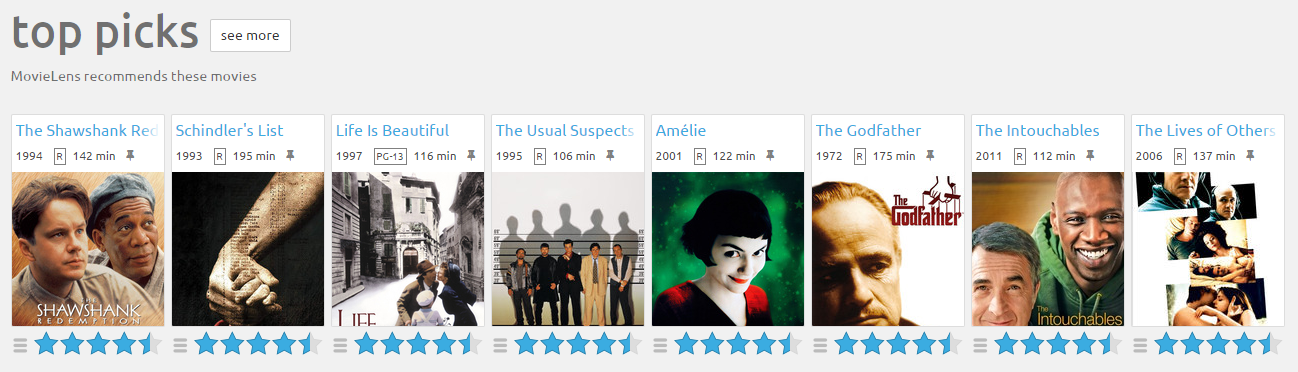
\includegraphics[width=14.21cm]{images/collaborative/movielens.png}
	\caption{Primjer preporuke sustava \glqq MovieLens\grqq}
	\label{fig:movielens}
\end{figure}

Ovaj pristup je relativno efikasan i jednostavan za implementaciju, ali druge
strane, računalno postaje vrlo zahtjevan ako se primjeni na velike baze podataka
korisnika i predmeta. Računanje transponirane matrice u općem slučaju je
složenosti $O((n \ast (n-1)) / 2)$. Računanje Pearsonovog koeficjenta korelacije
između svih korisnika iznosi $O(n^3 / 2)$ jer je složenost računa $O(n)$, a
potrebno je izvesti račun za gornji trokut kvadratne matrice širine $n$. Na
kraju složenost računa normaliziranog prosjeka iznosi $O(n * s)$ gdje je $s$
veličina susjedstva. Naposlijetku algoritam \ref{algo:korisnik-korisnik} daje
složenost:
\begin{equation}
\label{eq:slozenostKorisnik}
	O(
		\frac{n \ast (n-1)}{2} + 
		\frac{n^3}{2} + 
		(n \ast s)
	) = O(n^3)
\end{equation}

Ocjena \ref{eq:slozenostKorisnik} ima kvadratnu ovisnost i s povećanjem broja
korisnika dolazi do nemalog povećanja broja operacija za izračun preporuke. 
Valja dodati i da je algoritam \ref{algo:korisnik-korisnik} pojednostavljena
verzija algoitma, pa ni ocjena \ref{eq:slozenostKorisnik} ne može biti uzeta
kao konačna.

\subsubsection{Predmet -- Predmet}
S obzirom na nedostatke prethodne tehnike u performansama, inženjeri poznate
internetske trgovine \emph{Amazon.com} predložili su sličan pristup ali iz druge
perspektive gdje se ne traže sličnosti između korisnika, nego između predmeta
\cite{amazon}. Kao i kod prethodno opisanog pristupa i algoritma
\ref{algo:korisnik-korisnik}, metrika za ocjenu sličnosti između predmeta je
Pearsonov koeficjent korelacije, u ovom slučaju definiran kao:

\begin{equation}
\label{eq:pearsonPredmet}
	R = \frac
			{\sum_{u \epsilon U} 
				\big[
					(r_{u,i} - \overline{r_i}) \ast
					(r_{u,j} - \overline{r_j})
				\big]
			}
			{
				\sqrt{{\sum_{u \epsilon U} (r_{u,i} - \overline{r_i})^2}} \ast 
				\sqrt{{\sum_{u \epsilon U} (r_{u,j} - \overline{r_j})^2}}
			}
\end{equation}

gdje je $U$ skup svih korisnika koji su ocjenili predmete $i$ i $j$, $r_{u,i}$
ocjena korisnika $u$ za predmet $i$, a $\overline{r_i}$ srednja ocjena $i$-tog
predmeta za sve korisnike. Radi jednostavnosti, kod ovog algoritma matrica
ocjena korisnika za predmete normalizira se oduzimanje prosječne ocjene
kojom je svaki korisnik ocjenio predmete. 

Slično kao i kod suradnje na razini Korisnik-korisnik, predviđanje ocjene
korisnika $k$ za predmet $i$ računa se korištenjem težinskog prosjeka:
\begin{equation}
\label{eq:tezinskiProsjek}
	p_{k,i} = 
		\frac
			{\sum_{j \epsilon N} r_{k,j} \ast w_{i,j}}
			{\sum_{j \epsilon N} \|w_{i,j}\|}
\end{equation}
gdje je $N$ susjedstvo predmeta ocjenjenih od strane korisnika $k$ najsličnijih
predmetu $i$.

algoritam

Jedan od najpoznatijih preporučitelja na svijetu, internetska
trgovina \emph{Amazon.com} koristi patentirani hibridni algoritam baziran na
ovoj tehnici (slike \ref{fig:amazon1} i \ref{fig:amazon2}).
\begin{figure}[!htb]
	\centering
	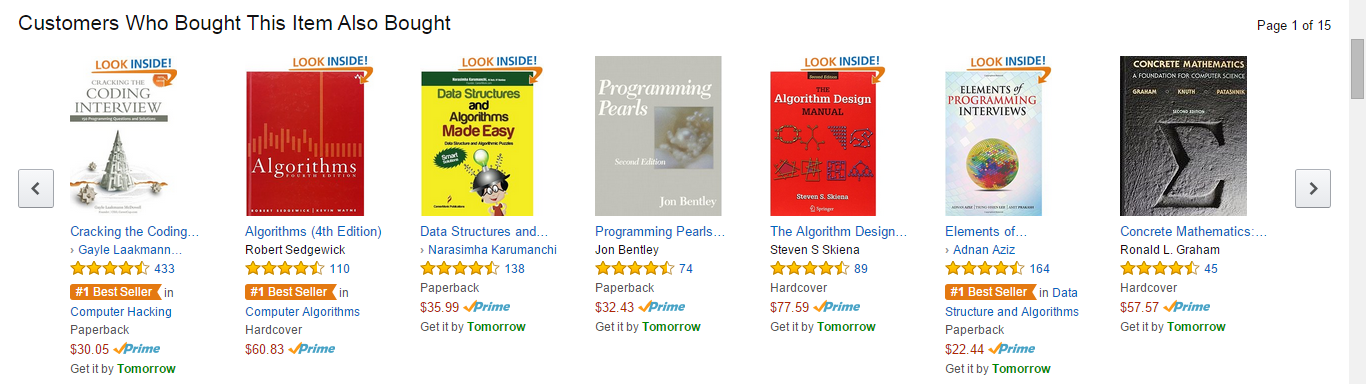
\includegraphics[width=14.21cm]{images/collaborative/amazon.png}
	\caption{Primjer preporuke sustava \glqq Amazon.com\grqq}
	\label{fig:amazon1}
\end{figure}

\begin{figure}[!htb]
	\centering
	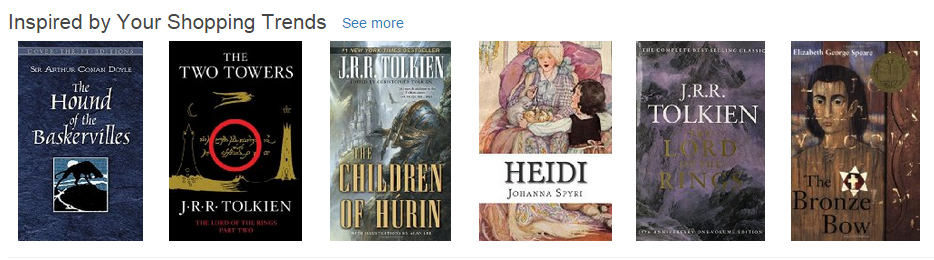
\includegraphics[width=14.21cm]{images/collaborative/amazon2.png}
	\caption{Primjer preporuke sustava \glqq Amazon.com\grqq}
	\label{fig:amazon2}
\end{figure}

\section{Redukcija dimenzija}


\section{Hibridne tehnike}
Hibridne tehnike podrazumjevaju kombiniranje više različitih tehnika filtriranja

zbog pokrivanja većeg spektra
kombiniranje kvalitetnijih obilježja u nekim okolinama
performanse

\begin{enumerate}
  \item Težinski - ocjena predmeta preporuke računa se iz svih dostupnih
  preporučiteljskih tehnika u sustavu. Najjednostavniji primjer jest linearna
  kombinacija preporuka. Neki sustavi koji koriste ovu tehniku kombiniraju
  preporuke zasnovane na suradnji i preporuke zasnovane na sadržaju uz
  kalibraciju težina u ovisnosti o povratnoj informaciji korisnika.
  \item Izmjenični - kod ove tehnike sustav koristi neki predefinirani kriterij
  za izmjenu tehnike preporuke, primjerice, neka je dan sustav koji inicijalno
  za svakog korisnika koristi preporuku zasnovanu na suradnji. Ako sustav tom
  tehnikom ne može stvoriti preporuku određenog nivoa pouzdanosti, rpebacuje se
  na preporuku zasnovanu na sadržaju.
  \item Miješani - ova tehnika računa preporuke iz više elementarnih
  preporučitelja i prikazuje ih simultano.
  \item Kombinacija obilježja - jedan od načina za spajanje suradnjičkog i
  sadržajnog preporučitelja jest interpretirati informacije suradničkog
  preporučitelja kao dodatne podatke koji čine ulaz sadržajnog preporučitelja.
  \item Kaskada - ova tehnika predstavlja svojevrsnu dvorazinsku preporuku. Prvo
  jedan preporučitelj relativno grubo rangira potencijalne kandidate, a nakon
  toga drugi preporučitelj radi precizniju razdiobu. Tehnika je posebno pogodna
  za one slučajeve kada jedan preporučitelj ne može dovoljno precizno generirati
  predviđanja za preporuke predmeta.
  \item Pojačavanje obilježja - tehnika kod koje je generirano predviđanje ili
  klasifikacija predmeta jednog preporučitelja pripojena slijedećoj
  preporučiteljskoj tehnici u nizu.
  \item Meta razina - izlaz jednog preporučitelja je ulaz drugog preporučitelja.
\end{enumerate}

Konkretne primjene preporučiteljskih sustava u heterogenim okolinama, danas se
svode u velikoj mjeri na različite hibride osnovnih tehnika. Velike industrije
trgovine i zabavnih sadržaja u praksi imaju autorska algoritamska rješenja
hibridnih preporučitelja.
\section{Moguća područja primjene}
utrpaj iz seminara


\section{Preporučiteljski sustavi u sveprisutnom računarstvu}
Primjena preporučiteljskih sustava u sveprisutnom računarstvu logična je
posljedica ne samo činjenice da je sveprisutno računarstvo računarstvo kao takvo
pa u njemu postoji interes za preporukom, nego i činjenice da se u njemu
generiraju velike količine podataka pa se preporučiteljski algoritmi mogu
primjeniti kao filtri podataka. O podacima sveprisutnom računarstvu praktički
je nemoguće govoriti bez konteksta u kojem se nalaze. Taj kontekst može se
definirati kao bilo koja informacija o okolnostima, predmetima ili uvjetima
koje okružuju korisnika, a smatra se relevantnom za interakciju između
korisnika i sveprisutnog računalnog okruženja \cite{RanganathanCampbell}.

Tri najvažnija aspekta kontekseta su \cite{schilit1994context}:
\begin{enumerate}
  \item Gdje se korisnik sustava nalazi
  \item U društvu kojih je drugih korisnika sustava
  \item Koji resursi se nalaze u blizini
\end{enumerate}

Koje su specifičnosti? Nisam ni sam ziher, algoritam vjerojatno mora biti
prilagođen filtiranju ogromne količine nestrukturiranih podataka, kontekst
vremena i prostora je najbitniji, predmeti preporuke su iz puno više različitih
domena nego npr na amazonu, pa ih je teže opisati.

Primjer preporučiteljskog sustava koji se djelomično nalazi u sveprisutnom
računarstvu jest algoritam koji koristi \emph{Foursquare}. \emph{Foursquare} je
servis koji preporučuje lokale na temelju preferencija korisnika, njegovih
ocjena sličnih lokacija te ocjena njegovih najbližih prijatelja i stručnjaka
koje prati \cite{FoursquareAbout}. Kod ovog preporučitelja vidljiv je prostorni
kontekst u smislu preporučivanja

specifičnosti, koji postoje, mobilni uređaji, foursquare itd.
%-------------------------------------------------------------------------------
%  CHAPTER: Izgrađeni model preporučiteljskog sustava
%-------------------------------------------------------------------------------
\chapter{Izgrađeni model preporučiteljskog sustava}


\section{Preporučiteljski sustavi s izraženom prostornom i vremenskom
komponentom}

Priča o postojećim preporučiteljima i kako nemaju prostorno vremenskih
komponenti 

Osnovni problem s kojim se konvencionalni preporučiteljski sustavi susreću (a
time i popularniji radni okviri i biblioteke koji ih implementiraju) jest
izostanak bilo kakve potpore za prostorne i vremenske komponente koje
su se pokazale neophodne za rad sa sveprisutnim sustavima. 
%Za sveprisutno prostor i vrijeme su jedne od bitnijih stavki (referenca?)

\section{The model}
Znači cijeli model treba opisati, od ocjenjivanja do apsolutno svega

\begin{equation}
\label{eq:DefModel}
	R \leftarrow U \times I \times C
\end{equation}

\begin{equation}
\label{eq:Context}
	C \leftarrow T \times S
\end{equation}

Izražen prostorno vremenski kontekst (općenito)
dvije razine reinforcementa. preporučitelj neće raditi online, tj. akcije iz
trenutnog sessiona ne utječu na preporuke u tom istom sessionu. tek kad se
session commita (po izlasku iz sustava) profili se zbrajaju i preporuke postaju
aktualne koje je pravo vrijeme za reinforcement dva profila -> privremeni i
trajni profil pa zbroj nakon kupnje netko svaka dva tjedna kupuje jabuke pa mu
se svaka dva tjedna kupuju jabuke (recurring)


Tu bi u principu trebalo ubaciti the algoritam
* fade out efekt
akcije(u konzumu)
I kolaboracija i sadržaj
- kod sadržaja, gdje je udaljenost manja od nekog broja (i fizička udaljenost)
- račun udaljenosti je apstrahiran

Možda sekcija kontekst pa onda napisati nešto generički o kontekstu pa onda
podsekcije prostor i vrijeme
Sekcija za svaku komponentu, korisnika i predmete, fino opisati od čega se
sastoje itd.

Kakve su ocjene, koje su skale

\begin{algorithm}[!htbp]
	\caption{Algoritam kontekstualizirane preporuke u vremenu i prostoru}
	\label{algo:TheAlgo}
	\begin{algorithmic}[1]
		\STATE{\textbf{Ulaz: Korisnik $u$, Prostor $l$, Vrijeme $t$} }
		\STATE{\textbf{Izlaz: Vektor kretanja $v$} }
		
		\FOR{($i := 0; i < n; inc(i)$)}
			\STATE{$w_i := calculatePearson(k, N_i)$}
		\ENDFOR
		
		\STATE{sort(w)}
		\STATE{$suma := 0; tezine := 0$}
		
		\FOR{($i := 0; i < topN; inc(i)$)}
			\STATE{$suma := suma + w_i * N_i$}
			\STATE{$tezine := tezine + w_i$}
		\ENDFOR
		
		\STATE{$p := suma / tezine$}
		
		\RETURN{p}
	\end{algorithmic}
\end{algorithm}

\begin{enumerate}
  \item Prostorni filter: sve što je trenutno u okolini korisnika manje od
  nekog graničnog „radiusa“, uzmi u obzir, ostalo odbaci. Potrebno između
  ostalog da smanjimo broj računanja. Što je veća blizina, to veća težina u
  rezultatu. Tu ide definicija udaljenosti, ili graf pa
  Dijkstra/Bellman-Ford/A*, ili kvadradna mreža pa Manhattan distance
  
  \item Vremenski filter: Uzeti u obzir dio dana i dio tjedna, što smo
  vremenski bliže vremenu u kojem korisnik kupuje te predmete, to je veća
  težina/utjecaj. Svaki korisnik ima funkcije (kontinuirane ili diskretne)
  kojima se opisuje vremenska preferencija za neke predmete
  
  \item U ovoj fazi postoji lista s poredanim prostorno vremenskim
  „udaljenostima“. Ako sadrži manje od nekog broja predmeta, ponovi od 1. ali
  olabavi kriterije
  
  \item U ovoj fazi primjenjujemo prilagođeni kolaborativni i content filter.
  Može i SVD dekompozicija(skupo) pa matrična algebra
  
  \item Imamo listu, sortira se prema lokaciji i vodimo korisnika. Može se
  izvesti da se kao težine putova označe rezultati predikcije pa se zavrti još
  jednom Dijkstra i imamo putanju.
  
\end{enumerate}

\section{Prostorna komponenta}

S obzirom na kompleksnost postupka modeliranja prostora, prostorna komponenta
konteksta modelirat će se poednostavljeno, i to kvadratnom mrežom
(slika \ref{fig:StoreGrid}). Iako se na prvi pogled tako čini, to nije
ograničenje jer modeliranje prostora u kojem će korisnici tražiti preporuku
najčešće nije slobodno, tj. korisnik se u takvim prostorima kreće putem koji mu
je dostupan. Primjer je dućan u kojem se korisnik može kretati između polica, a
očito je i razumno da se ne može kretati \emph{preko} polica.
%TODO: ružno napisano, refactor
Dostupne puteve za korisnika može se čuvati u npr. riječnicima
\engl{Dictionary}, tj. parovima $kljuc \rightarrow vrijednost$ gdje je $kljuc$
neko polje kvadratne mreže a $vrijednost$ lista svih \emph{susjednih} polja do
kojih je moguće doći iz polja $kljuc$. Minorna mana ovog pristupa jest
dvostruko spremanje putova jer ako se iz polja $p_1$ može doći u polje $p_2$,
onda se iz polja $p_2$ može doći u polje $p_1$. Dvostruko spremanje može se
izbjeći nauštrb vremenu pretraživanja dvostrukih putanja, a za relativno malu
memorijsku uštedu, čak i kod modeliranja vrlo velikih prostora.
%TODO: Manhattan distance
%TODO: refactor text
Ako se kvadratnu mrežu i dostupne putove kretanja prikaže kao neusmjereni
težinski graf, onda se taj prostor može predstaviti \emph{matricom
susjedstva}, a kako je takva matrica simetrična, spremati se može samo npr.
gornja trokutasta matrica, čime se postiže svojevrsna rijetka popunjenost
matrice \engl{Sparse Matrix}.
%TODO: i ovo refactor
%treba napisati kako su različite namjene dijkstre i A* itd.
Prednost predstavljanja mreže i prostora grafom jest i postojanje nebrojeno
mnogo pouzdanih i efikasnih algoritama za traženje najkraćeg puta između dva
vrha, odnosno dva polja. Neki od njih su npr. \emph{Dijkstrin algoritam},
\emph{Bellman-Ford algoriam} ili \emph{A$\ast$ algoritam}.

\begin{figure}[!htb]
	\centering
	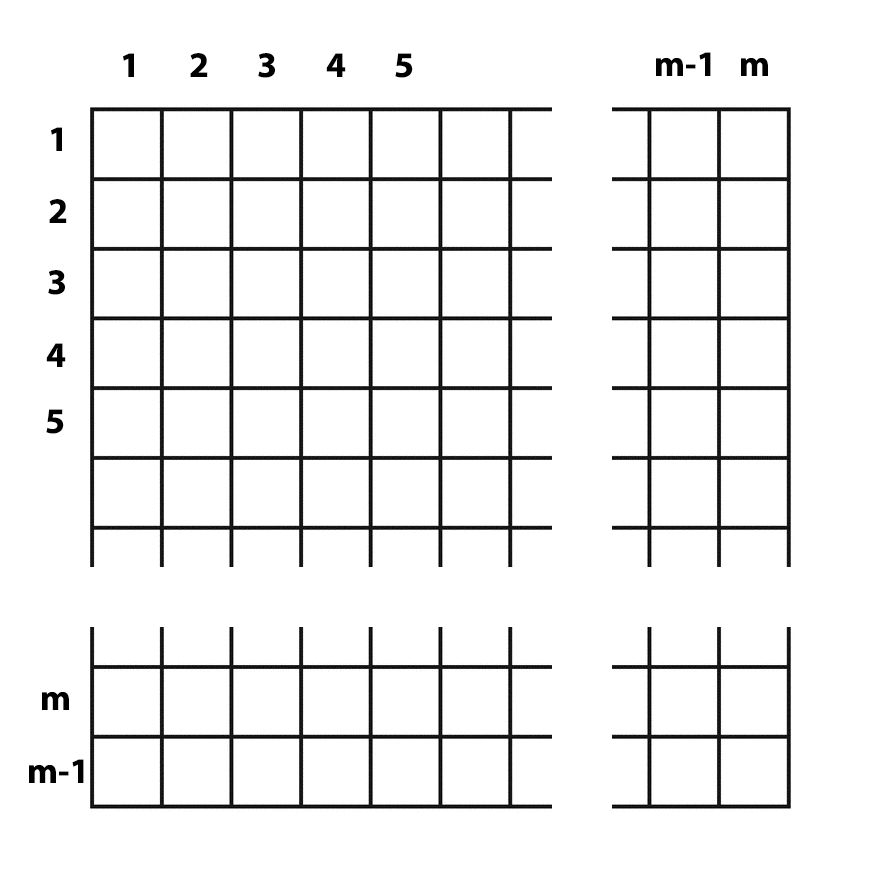
\includegraphics[width=7cm]{images/grid.png}
	\caption{Tlocrt prostora modeliran kvadratnom mrežom}
	\label{fig:StoreGrid}
\end{figure}

\begin{figure}[!htb]
	\centering
	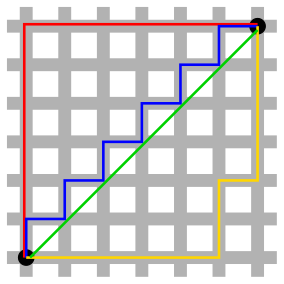
\includegraphics[width=7cm]{images/Manhattan_distance.png}
	\caption{Ilustracija Manhattanske udaljenosti}
	\label{fig:ManhattanDistance}
\end{figure}



\section{Vremenska komponenta}

Vremenska komponenta koja se uzima u obzir u modelu preporučitelja također je
zapravo komponenta konteksta u kojem se nalazi korisnik. 

uuuu, korisnik može za određeni proizvod imati funkciju koja opisuje kakve on
ima vremenske preferencije s obzirom na taj proizvod. ili funkcija može
opisivati samo one trenutke kada se stavlja korisnik u situaciju da traži
preporuk

Jedna takva funkcija može biti primjerice tzv. \emph{Gaussova krivulja}
(slika \ref{fig:Gauss1}). Ona je pogodna zbog činjenice da prosječan korisnik
prosječnu akciju u kojoj će tražiti preporuku u principu traži u jednom kraćem
vremenskom intervalu. Drugim riječima, pojedini predmeti preporuke za nekog
korisnika u vremenski svjesnom preporučiteljskom sustavu bit će zanimljivi samo
jedan kraći interval.
\begin{equation}
	\label{eq:BellFunc}
	f(x;a,b,c) = \frac
	{
		1
	}
	{
		1 + \mid\frac{x - c}{a}\mid^{2b}
	}
\end{equation}
gdje je $x$ varijabla, a $a$, $b$ i $c$ parametri kojima se regulira oblik
krivulje:
\begin{itemize}
  \item $a$ - širina vrha
  \item $b$ - nagib porasta i pada, oblik vrha
  \item $c$ - pomak na $x$ osi
\end{itemize}

\begin{figure}[!htb]
	\centering
	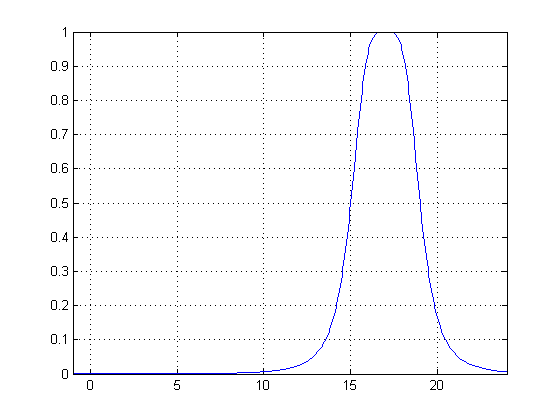
\includegraphics[width=12cm]{images/zvonolika1matlab.png}
	\caption{Preferencija korisnika za predmet na dnevnoj skali}
	\label{fig:Gauss1}
\end{figure}

S druge strane, skala ne mora biti dnevna, može biti i tjedna te se funkciju
može zadati po dijelovima (puno kompleksnije situacije). 
Znači, funkcija može biti na više različitih skala i može odražavati
preferenciju za predmet ili preferenciju za traženje preporuke općenito
%TODO Tu mi fali neka slika funkcije pod više dijelova i na tjednoj skali
\begin{figure}[!htb]
	\centering
	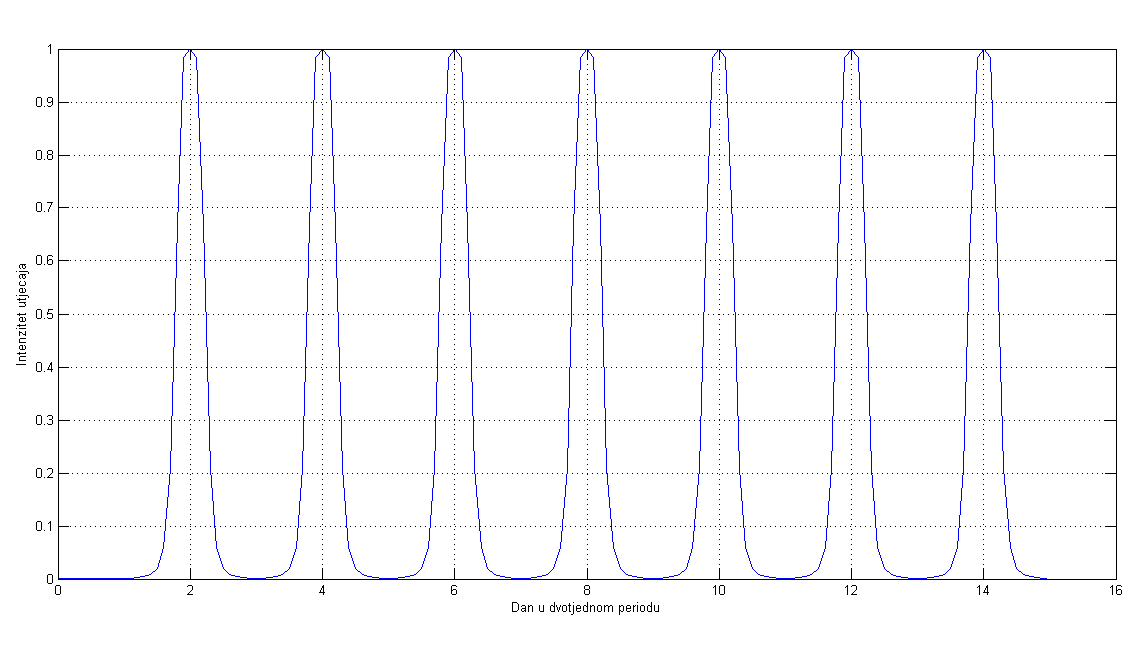
\includegraphics[width=14.21cm]{images/neprigusenocropped.png}
	\caption{Preferencija korisnika za predmet na dnevnoj skali}
	\label{fig:Gauss2}
\end{figure}

S obzirom na matematičku analizu koja stoji iza računa za pronalazak funkcije,
one se mogu zadati i diskretno, npr. kroz vektor uzoraka funkcije. Ta diskretnu
funkciju može se koristiti kao takva ili se može procesom interpolacije naći
njezin eksplicitni zapis. Pogodne metode interpolacije mogu npr. biti
interpolacija polinomom višeg stupnja ili interpolacija splajnovima
\engl{Spline}.

u funkcija može biti kontinuirana, a može biti i uzorkovana i
pohranjena u nekom polju. y os funkcije tada je vrijednost koju korisnik
pridaje nekom proizvodu u neko doba dana. ne mora biti ni doba dana, može biti
doba tjedna. diskretizirane funkcije mogu se interpolirati polinomima višeg
stupnja ili splajnovima

%TODO: refactor
Vremenska komponenta omogućava i praćenje obrazaca ponašanja korisnika, pa time
i predviđanje ponavljanja ponašanja \engl{Recurring}.

Vremenska komponenta podrazumjeva i tzv. \emph{efekt blijeđenja} \engl{Fade-out
effect}. Ako korisnik kod kojeg je uočen neki obrazac akcija prestane provoditi
tu akciju, preporučitelj će prestati primati pobudu za održavanje te akcije.
Međutim, neće je odmah zanemariti nego će se vremenska komponenta, tj. funkcija
koja opisuje tu komponentu, lagano gušiti nekom drugom funkcijom, primjerice
recipročnom eksponencijalnom funkcijom:

\begin{equation}
	\label{eq:RecipExp}
	g(x) = e^{-x}
\end{equation}

Tada će ukupan rezultat vremenske komponente konteksta biti:

\begin{equation}
	\label{eq:Gusenje}
	T \leftarrow f(x) \ast g(x)
\end{equation}

gdje je $f(x)$ funkcija koja opisuje vremensku komponentu konteksta nekog
korisnika za neki predmet, a $g(x)$ funkcija koja guši tu komponentu.
primjer. 

Na slici \ref{fig:GaussPriguseno} vidljiv je primjer \emph{efekta
blijeđenja} na tipično periodičko ponašanje korisnika. Prema formuli
\ref{eq:Gusenje} vrijedi:

\begin{equation}
	\label{eq:BellFunc}
	f(x) = \frac
	{
		1
	}
	{
		1 + \mid\frac{x - 2*k}{0.23}\mid^{5}
	}
	+ 2 \ast k + 1
\end{equation}
gdje je $k \in \{ 0, 1, 2, 3, 4, 5, 6, 7 \}$

\begin{equation}
	\label{eq:Prigusnica}
	g(x)=e^{-0.18 * x}
\end{equation}

Ovdje također postoji mogućnost da se funkcija $g(x)$ zada diskretno, tj. po
uzorcima.

%TODO: slika s gušenjem
\begin{figure}[!htb]
	\centering
	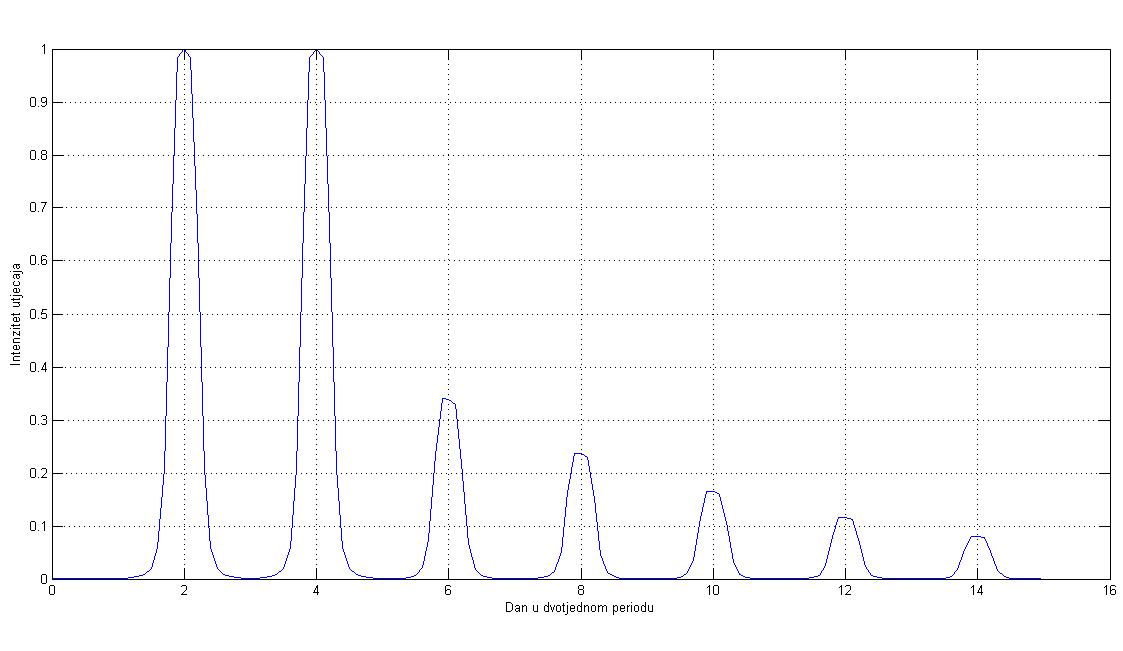
\includegraphics[width=14.21cm]{images/prigusenocropped.png}
	\caption{Preferencija korisnika za predmet na dnevnoj skali}
	\label{fig:GaussPriguseno}
\end{figure}

akcije

\section{Modeliranje korisnika}
multiplus profil

\begin{enumerate}
  \item multiplus profil, znamo tko što voli, tj. imamo profil korisnika
  \item dopuna profila? kroz šetnju, kroz zadržavanje, kada kupi?
  \item cold start profil?
\end{enumerate}

Profil:
\begin{enumerate}
  \item Proizvodi, skupine proizvoda, redovi? -> stablo?
  \item vektor preferencija
\end{enumerate}

\section{Modeliranje predmeta}

%Novi chapter%
\chapter{Implementacija i ispitivanje modela}
\section{Arhitektura implementacije}
Opisati razrede, lupiti negdje class diagram itd.

\section{Ispitni scenarij}
Osmišljavanje ispitnog scenarija pokazalo se natprosječno zahtjevnim radi
pokušaja da takav scenarij obuhvati i ispita sve segmente kontekstualno svjesnog
preporučitelja. S druge strane, takav scenarij je morao biti realno
ostvariv, u smislu da ne bude sintetički osmišljen nego da u realnom
svijetu postoji takva situacija u kojoj će se osmišljeni preporučiteljski
model moći implementirati i koristiti. Na kraju je odabrana prosječna
svakodnevna aktivnost većine potencijalnih korisnika ovakvog sustava, a to je
odlazak u kupovinu.

Ispitni scenarij podrazumjeva generički srednje velik dućan u kojem se
može naći mješovita roba, dakle, i prehrana i neprehrana. Radi jednostavnosti, a
bez značajnijeg utjecaja na krajnji ishod, tlocrt dućana modeliran je mrežastom
strukturom prikazanom na slici \ref{fig:StoreGrid}. U dućanu se na svakom mjestu
mogu nalaziti radio oznake \engl{beacon} kojima mogu biti obilježeni:
\begin{itemize}
  \item Neka lokacija u dućanu, npr. red polica
  \item Skupina proizvoda
  \item Konkretan proizvod
\end{itemize}
Ovdje se nameće pitanje je li potrebno radio oznakama obilježiti sve
potencijalne predmete preporuke. Sa strane sustava, podrazumjeva se
posjedovanje točnih lokacija svake radio oznake, a poznavanjem točnih lokacija
te poznavanjem rasporeda u dućanu, interpolacijom se može aproksimirati lokacija
korisnika u trenutcima kada je on između radio oznaka. Svakoj radio oznaci
pridodani su i neki metapodaci od kojih je najvažniji jedinstveni identifikator
u sustavu.

%TODO: beacon opis
Svaka radio oznaka ima određeni domet signala kojim razašilje \engl{broadcast}
svoj jedinstveni identifikator. Kada se mobilni uređaj nađe u dometu signala, on
prima taj jedinstveni identifikator te može utvrditi \emph{RSS} \engl{Received
signal strength}. 

\begin{figure}[!htb]
	\centering
	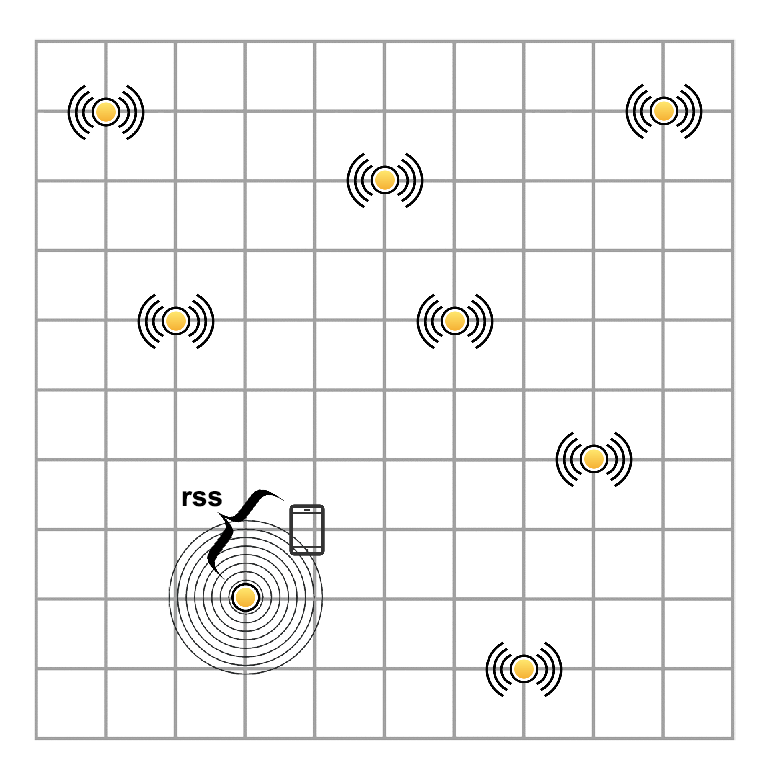
\includegraphics[width=9cm]{images/gridbeacons1cell.png}
	\caption{Grafički prikaz radio oznake i mobilnog telefona}
	\label{fig:RssOneCell}
\end{figure}

Slika \ref{fig:RssOneCell} prikazuje slučaj kada je mobilni
uređaj u dometu jedne radio oznake. U tom slučaju može se smatrati da je
korisnik zainteresiran za ono što radio oznaka obilježava. S druge strane,
ako se korisnik nađe u dometu dva ili više radio oznaka (slika
\ref{fig:RssTwoCells}), onda se jednostavno uzima signal one radio oznake čiji
je \emph{RSS} u tom trenutku jači. Naime, \emph{RSS} opada s udaljenošću pa se s
pravom može smatrati da jači \emph{RSS} nužno povlači veću fizičku blizinu
korisnika u odnosu na pripadajuću radio oznaku, tj. ono što ta radio oznaka
obilježava.

\begin{figure}[!htb]
	\centering
	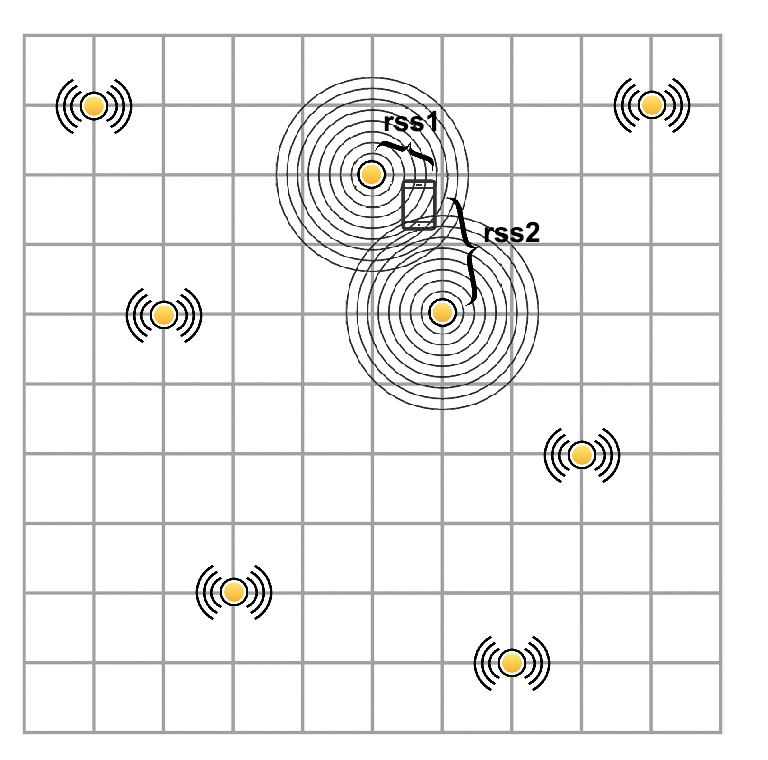
\includegraphics[width=9cm]{images/gridbeacons2cells.png}
	\caption{Grafički prikaz višestrukog prijama signala s radio oznaka}
	\label{fig:RssTwoCells}
\end{figure}

Također, uzima se u obzir i vrijeme zadržavanja korisnika u blizini radio
oznake. Ukoliko je korisnik proveo manje vremena od neke empirijski određene
vremenske granice $t_min$, onda se može smatrati da korisnik nije iskazao
interes za predmet koji radio oznaka obilježava.
U obzir valja uzeti i orjentaciju korisnika. Nerijetko je moguće da korisnik
bude u dometu signala radio oznake, a fizički nije usmjeren prema predmetu koji
ona označava. Korištenjem magnetometra na pametnom uređaju i poznavanjem
razmještaja radio oznaka u prostoru, može se jednostavno utvrditi je li korisnik
iskazao interes za obilježeni predmet ili je okrenut od njega.
%zadržavanje -> reinforcement prvog stupnja

Izvor podataka je dobro enkapsuliran pa se može reći da mora implementirati
sučelje s određenom opremom, a ta oprema je:
\begin{itemize}
  \item Komunikacijski radio, npr. \emph{WLAN} \engl{Wireless LAN} -- koristi
  se za svu komunikaciju sa poslužiteljima po pitanju dohvaćanja metapodataka o
  radio oznakama, traženje preporuke itd.
  \item Magnetometar -- koristi se utvrđivanje je li korisnik okrenut prema
  radio oznaci ili od nje. % 
  \item Akcelerometar -- koristi se za utvrđivanje gibanja korisnika. Ako je
  korisnik u pokretu, zanemaruju se podaci sa ulaza za očitavanje radio oznaka
  \item Bluetooth -- koristi se za komunikaciju s radio oznakama
\end{itemize}

Takav izvor u praksi može biti bilo koji moderniji mobilni telefon ili tablet.

\section{Simulacija primjene}
U praktičnom smislu, ispitni scenarij modeliran je radio oznakom i prolaskom
korisnika s mobilnim telefonom. Korisnik hoda normalnim hodom prosječne brzine,
a mobilni telefon drži u ruci koja slobodno visi i giba se u skladu s koracima.
Radio oznaka razašilje jedinstveni identifikator frekvencijom od $1 Hz$, a
mobilni telefon bilježi podatke frekvencijom od $5 Hz$. Različite razine
povratne informacije preporučitelju o akcijama korisnika simulirane su
različitim ponašanjem u ispitnom scenariju, a vidljive su u tablici
\ref{tbl:podscenariji}

\begin{table}[!htb]
	\caption{Ispitni podscenariji}
	\label{tbl:podscenariji}
	\centering
	\begin{tabular}{|c|c|c|} \hline		
		Dataset & Način zaustavljanja & Korištenje mobitela\\ \hline
		1 & Ne postoji & Ne\\
		2 & Usporavanje & Ne\\
		3 & Zastajkivanje & Ne\\
		4 & Zastajkivanje & Kraće podizanje\\
		5 & Zastajkivanje & Dulje podizanje\\
		6 & Zaustavljanje & Ne\\
		7 & Zaustavljanje & Kraće podizanje\\
		8 & Zaustavljanje & Dulje podizanje\\ \hline
	\end{tabular}
\end{table}

Tablica \ref{tbl:reinforcement} prikazuje konkretne iznose odgovora na različite
pobude od strane korisnika na sustav.

\begin{table}[!htb]
	\caption{Reakcije na interakciju korisnika i predmeta}
	\label{tbl:reinforcement}
	\centering
	\begin{tabular}{|c|c|} \hline		
		Način zaustavljanja & Pojačanje\\ \hline
		Ne postoji & 0\\
		Usporavanje & 0.025\\
		Zastajkivanje & 0.05\\
		Zaustavljanje & 0.1\\ \hline
	\end{tabular}
\end{table}

%Kako se konkretno računa zaustavljanje, usporavanje zastajkivanje itd.

\subsection{Ulazi}
Ulazi u sustav ugrubo se mogu podijeliti na ulaze potrebne za postavljanje
sustava i ulaze na koje sustav reagira preporukom. Ulazi potrebni za
postavljanje su tlocrt, tj. prostorni opis okoline, podaci o ocjenama korisnika
sustava za predmete, predmeti sustava sa vektorima svojih karakteristika te
podaci o vezama između radio oznaka i predmeta. Uz navedene podatke, ulaz u
sustav je i jedinstveni identifikator korisnika za kojeg se traži preporuka. Taj
identifikator jest jednostavan podatak cjelobrojnog tipa pa neće biti detaljnije
opisivan. Također, ulaz u sustav je i cijeli broj $N$ kojim se specificira
koliko se najboljih predmeta traži za korisnika.

\subsubsection{Prostorni opis okoline}
Za potrebe testiranja koristi se jednostavni generirani tlocrt prikazan slikom
\ref{fig:layout}. Razlog relativno jednostavnom tlocrtu jest kombinatorna
eksplozija kojoj su veći prostori podložni. Tlocrt se učitava iz \emph{CSV}
datoteke \engl{Comma separated values}, a u toj datoteci zapisana je matrica
susjedstava grafa (\ref{eq:adjacencyMatrix}) koji odgovara tlocrtu. Zbog
jednostavnosti, praktično je tlocrt prikazati grafom zbog velikog broja
dostupnih i provjerenih algoritama za izračun udaljenosti između čvorova

\begin{figure}[!htb]
	\centering
	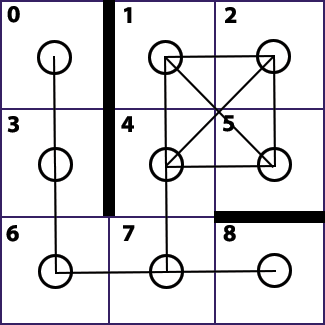
\includegraphics[width=5cm]{images/3x3grid.png}
	\caption{Jednostavan ispitni tlocrt}
	\label{fig:layout}
\end{figure}

\begin{equation}
	\label{eq:adjacencyMatrix}
	M = 
	\begin{bmatrix}
		0 & 0 & 0 & 1 & 0 & 0 & 0 & 0 & 0\\
		0 & 0 & 1 & 0 & 1 & 1 & 0 & 0 & 0\\
		0 & 1 & 0 & 0 & 1 & 1 & 0 & 0 & 0\\
		1 & 0 & 0 & 0 & 0 & 0 & 1 & 0 & 0\\
		0 & 1 & 1 & 0 & 0 & 1 & 0 & 1 & 0\\
		0 & 1 & 1 & 0 & 1 & 0 & 0 & 0 & 0\\
		0 & 0 & 0 & 1 & 0 & 0 & 0 & 1 & 0\\
		0 & 0 & 0 & 0 & 1 & 0 & 1 & 0 & 1\\
		0 & 0 & 0 & 0 & 0 & 0 & 0 & 1 & 0\\
	\end{bmatrix}
\end{equation}

U datoteci u kojoj je tlocrt zapisan, elementi stupaca matrice odvojeni su
znakom točka - zarez \engl{Semicolon}, a elementi redaka znakom novog retka.
Datoteka se procesira na početku rada sustava, a po potrebi svaki put kada se
dogodi promjena rasporeda u prostoru. U tom slučaju, pretpostavlja se da će u
datoteci biti zapisan novi tlocrt prostora.

\subsubsection{Veza između radio oznaka i predmeta}
Veza između radio oznaka i predmeta razmjerno je jednostavna. Također se učitava
iz \emph{CSV} datoteke, a format joj je:

\begin{equation}
	\centering
	beaconId;itemId
\end{equation}

S obzirom da izmjena radio oznake za neki predmet nije česta radnja, datoteka se
procesira jedanput na početku rada sustava. U slučaju promjena, nove podatke
moguće je unijeti dinamički u sustav.

\subsubsection{Podaci o predmetima}
Podaci o predmetima učitavaju se iz \emph{CSV} datoteke. Opći izgled retka
datoteke je:

\begin{equation}
	\centering
	itemId;itemName;locationId\#CharName1;CharName2 \ldots
\end{equation}

Prvo se čita prvi redak datoteke iz kojeg se nakon razdvajanja učitanog retka po
znaku $\#$ prebrojavaju i učitavaju imena karakteristika kojima će se opisivati
predmeti. Karakteristika u sustavu može biti neograničeno mnogo. Nakon toga
slijedi slijedno čitanje datoteke, redak po redak. Svaki redak započinje
cijelim brojem koji je jedinstveni identifikator predmeta u sustavu. Nakon
njega, odvojen točka-zarezom slijedi naziv predmeta te cijeli broj koji je
jedinstveni identifikator lokacije, tj. ćelije, u sustavu. Nakon
znaka $\#$ slijedi niz sastavljen od $0$ ili $1$ odvojen znakom točka-zarez.
Znak $0$ označava da ta karakteristika nije prisutna u predmetu kojem pripada
redak, a znak $1$ da je karakteristika prisutna, tj. primjenjiva na predmet.

Nakon inicijalnog čitanja datoteke, nove predmete u sustav moguće je unijeti
dinamički. Primjer ove datoteke nalazi se u dodatku.

\subsubsection{Matrica ocjena korisnika}
Matrica ocjena korisnika također razlikuje prvi redak od ostalih. 
Oblik prvog retka datoteke je:
\begin{equation}
	\centering
	;itemId\#itemName;itemId\#itemName
\end{equation}
gdje predmeta može biti nedefinirano mnogo. Općeniti izgled ostalih redaka je:
\begin{equation}
	\centering
	userId;ratingForItem1;ratingForItem2 \ldots
\end{equation}
gdje je $userId$ jedinstveni identifikator korisnika u sustavu, a
$ratingForItem$ ocjena korisnika za predmet kojem odgovara stupac u kojem se ta
ocjena nalazi. Ocjene su predstavljene skupom:
\begin{equation}
	\centering
	R \in \big[ 0.5, 5.0 \big]
\end{equation}
Općenito, granulacija dodjeljivanja ocjena jest $0.5$ iako to nije kriterij za
stabilan rad sustava. Ukoliko ocjena korisnika za neki predmet ne postoji, pri
obradi retka, na to mjesto umeće se numerička oznaka $-100.0$ koja se naravno
ne koristi kao ocjena nego kao oznaka neodstatka ocjene. Primjer ove datoteke
može se naći u dodatku

\subsubsection{Dnevnički zapisi mobilnog uređaja}

%17:37:47.392#74278bda-b644-4520-8f0c-720eaf059935-baba-bebe$-86#9.8;-1.8;1.6#-42.2;4.7;13.9
Krajnji ulaz u sustav, bez ikakve apstrakcije, su dnevnički zapisi \engl{Log} s
pametnog uređaja. U njih uređaj zapisuje:
\begin{itemize}
  \item Vremensku oznaku
  \item Jedinstveni identifikator radio oznake
  \item \emph{RSS} \engl{Received signal strength}
  \item Podatke s mjerača ubrzanja \engl{Accelerometer}
  \item Podatke s magnetometra \engl{Magnetometer}
\end{itemize}
Dnevnički zapisi se pišu i čitaju u, odnosno iz obične tekstualne datoteke u
predefiniranom formatu:
\begin{equation}
	\centering
	timestamp;beaconId\$rss\#accelerometer\#magnetometer\char`\\n
\end{equation}
gdje je $\char`\\n$ oznaka za novu liniju \engl{Line feed}
Podaci $beaconId$ i $rss$ su, tipski gledano, jednostavni, a $timestamp$,
$accelerometer$ i $magnetometer$ složeni.

\begin{itemize}
  \item Vremenska oznaka -- $sat:minuta:sekunda.stotinka$
  \item Mjerač ubrzanja -- $x;y;z$ - mjeri ubrzanje sile na tri fizičke osi
  uređaja u $m/s^2$, uključujući ubrzanje sile teže.
  \item Magnetometar -- $x;y;z$ - mjeri ambijentalno geomagnetsko polje na tri
  fizičke osi uređaja u $\mu T$
\end{itemize}

\subsection{Izlazi}

Izlazi iz sustava su serijalizirani $Java$ interni objekti $ItemPredictionLink$
slijedećeg oblika:
\begin{equation}
	\centering
	ItemPredictionLink\{ 
		itemId=N,
		prediction=P
	\}
\end{equation}
gdje je $itemId$ jedinstveni identifikator predmeta u sustavu, a $prediction$
predikcija ocjene korisnika za kojeg je preporuka zatražena za predmet s
identifikatorom $itemId$. Objekti su smješteni u jednostruko povezanoj listi, a
prethodno su sortirani padajućim redoslijedom prema predikciji. Rezultati rada
sustava kao objekti se ispisuju na standardni izlaz računala \engl{STDOUT}.


%TODO: treba negdje ubaciti kako se stvar može generalizirati


Inicijalizacija se jednom zavrti a onda se preporuke šibaju nonstop. Nakon
reinforcementa i izmjene podataka, treba ponovno zavrtiti izračune korelacija i
ostalih content based gluposti.

\section{Rezultati testiranja}
Prikazati rezultate, jelte

\chapter{Zaključak}
Zaključak.

\bibliography{literatura}
\bibliographystyle{fer}

\begin{sazetak}
Sažetak na hrvatskom jeziku.

\kljucnerijeci{Ključne riječi, odvojene zarezima.}
\end{sazetak}

\engtitle{Recommender systems in ubiquituous computing}
\begin{abstract}
Abstract.

\keywords{Keywords.}
\end{abstract}

\appendix
\chapter{Primjer dnevničke datoteke}
\lstinputlisting[
		language=C, 
		firstline=37,
		lastline=46, 
		numbers=left, 
		breaklines=true, 
		numbersep=5pt,
		numberstyle=\color{mygray}
	]{logs/LogFile_06-06-15_18_27a.txt}
	
\chapter{Datoteka s podacima o predmetima}
\lstinputlisting[
		language=C, 
		firstline=1,
		lastline=15, 
		numbers=left, 
		breaklines=true, 
		numbersep=5pt,
		numberstyle=\color{mygray}
	]{csv/items.csv}

\chapter{Datoteka s matricom ocjena korisnika}
\lstinputlisting[
		language=C, 
		firstline=1,
		lastline=15, 
		numbers=left, 
		breaklines=true, 
		numbersep=5pt,
		numberstyle=\color{mygray}
	]{csv/ratings.csv}
	
\end{document}
